\vspace{-0.2cm}
The emergence of transformer \cite{vaswani2017attention} and its variants \cite{bai2020binarybert, devlin2018bert, hou2020dynabert} has catalyzed significant advancements in natural language processing (NLP), unveiling the immense potential for deploying NLP models on various devices.
The existing NLP paradigm encompasses two stages, \ie, pre-training and fine-tuning \cite{brown2020language, devlin2018bert}. 
Specifically, the language model (LM) is first pre-trained on a large corpus to learn general features and patterns. 
Subsequently, the LM is further fine-tuned on domain-specific data generated on devices to enhance the model performance for a specific task. 
However, it is infeasible to collect enough domain-specific data from devices for centralized fine-tuning due to data privacy \cite{mcmahan2017communication, lin2021fednlp, liao2023accelerating}. 
To fully utilize the massive data on devices, federated fine-tuning (FedFT) has been proposed to perform fine-tuning in a distributed manner \cite{lin2021fednlp}.
In the typical FedFT framework, \eg, FedNLP \cite{lin2021fednlp}, participating devices periodically fine-tune the LMs on their local data, and push the local LMs to the parameter server (PS) for global aggregation without exposing their raw data.
The fine-tuning procedure is repeated for multiple rounds until the LM converges or reaches the target accuracy \cite{mcmahan2017communication, stremmel2021pretraining, cai2022fedadapter}.
FedFT not only protects individual privacy but also fully utilizes plenty of computing resources on devices to enhance the fine-tuning performance of the LMs.

\textbf{Challenges of FedFT.}
Although FedFT has demonstrated its advantages, it still faces the following two challenges in practical applications: 
(1) \textit{Resource constraints}. 
Many devices such as smartphones and in-vehicle devices typically have limited resources (\eg, memory, computing power), which are orders of magnitude weaker than cloud servers \cite{xu2022adaptive, zhu2023pockengine, dhar2021survey, liao2024mergesfl}. 
However, existing LMs, \eg, Llama \cite{touvron2023llama}, typically involve billions of parameters, requiring substantial computing power for fine-tuning \cite{hu2021lora}, while resource-constrained devices always lead to very slow fine-tuning rates.
(2) \textit{System heterogeneity}.
The devices commonly possess varying computing capabilities (\eg, CPU frequency) or communication capabilities (\eg, bandwidth), which could differ from each other by more than tenfold \cite{liao2023adaptive, lai2021oort, liu2023yoga}.
Specifically, there are huge gaps of computing/communication capabilities among different types of devices, and even among devices of the same type with diverse configurations (\eg, smartphones, laptops) \cite{dhar2021survey}.
Due to system heterogeneity, fast devices should be forced to wait for slow ones, leading to prolonged waiting time and poor fine-tuning efficiency.

\textbf{Status Quo and Limitations.} 
To handle the issue of resource constraints, existing works rely on parameter-efficient fine-tuning methods \cite{zhang2023fedpetuning}, \eg, Adapter \cite{houlsby2019parameter} and low-rank adaptation (LoRA) \cite{hu2021lora}, which only fine-tune additional lightweight parameters (typically less than 1\%). 
The Adapter method inserts additional blocks between two continuous transformer layers and only updates the parameters of the inserted blocks to achieve efficient fine-tuning \cite{houlsby2019parameter}.
For example, Cai \etal \cite{cai2022fedadapter} first apply Adapter in FedFT and propose FedAdapter, which dynamically searches for the optimal Adapter structure to improve the fine-tuning efficiency.
However, the Adapter method inevitably brings additional inference latency, potentially resulting in up to a 30\% latency increase \cite{hu2021lora, liao2023parameter, li2024caraserve}, which is often unacceptable in practical applications, \eg, real-time sentiment analysis \cite{wankhade2022survey} and real-time news categorization \cite{minaee2021deep}. 
% \textbf{In addition, none of these methods have been tested under real wireless network environments where devices are heterogeneous and the network bandwidth of devices may vary over time.} 
In addition, none of these methods have been tested under real wireless network environments with heterogeneous devices. 


To avoid the extra inference latency, LoRA \cite{hu2021lora} has been proposed to freeze the pre-trained LM and add trainable bypass low-rank matrices (\ie, \textit{LoRA layers}) to the transformer layers, in which only the LoRA layers would be updated during fine-tuning.
The vanilla LoRA adds the LoRA layers with the \textit{same} rank (\ie, the dimension of the bypass low-rank matrices) to \textit{all} transformer layers \cite{zhang2022adaptive}.
To explore the potential of LoRA in FedFT, Zhang \etal \cite{zhang2023fedpetuning} propose FedLoRA and verify the efficiency of FedFT with vanilla LoRA through experiments.
Upon FedLoRA, Cho \etal \cite{cho2023heterogeneous} propose HetLoRA, in which each device adds LoRA layers to all transformer layers with a diverse and appropriate LoRA rank to deal with system heterogeneity.
However, due to the rank mismatch of all LoRA layers on different devices, it is difficult to aggregate these layers, resulting in poor fine-tuning performance.
In a nutshell, existing works simply add LoRA layers with the uniform rank distribution for all transformer layers, which still requires substantial computing and communication resources, resulting in slow fine-tuning speeds on weak devices.
Moreover, system heterogeneity further leads to low fine-tuning efficiency or poor fine-tuning performance \cite{kim2021autofl, luo2022tackling, liao2024mergesfl}. 
They do not address the two above challenges. 
% In conclusion, they fail to adequately address the two challenges mentioned above, leaving key issues unresolved in the context of the discussed approach.


\textbf{Overview of the Proposed Approach.} 
According to the pre-test in Section \ref{sec:prelim}, adding the LoRA layers with different LoRA configurations (\eg, LoRA depth and rank distribution) significantly impacts the fine-tuning performance and resource consumption, where LoRA depth denotes the number of the continuous LoRA layers from the output. 
Adding LoRA layers with higher ranks to transformer layers close to the output helps to save resource consumption while achieving comparable fine-tuning performance.
Based on the insight, we propose a novel FedFT framework with adaptive \textbf{L}oRA depth and rank distribution on h\textbf{e}tero\textbf{gen}eous \textbf{d}evices, termed LEGEND, to deal with resource constraint and system heterogeneity.
 % by jointly optimizing the LoRA depth and rank distribution
%The difficulty of system design lies in the interactions between LoRA depth and rank distribution. 
Our unique findings include: 1) 
large LoRA depth with high rank helps to achieve superior fine-tuning performance but incurs significant resource consumption, leading to a slow convergence rate on devices with limited resources; 2) Small LoRA depth with low ranks reduces the fine-tuning overhead on devices while resulting in poor fine-tuning performance or even failure to converge.
Therefore, it is necessary yet challenging to simultaneously determine the appropriate LoRA depth with reasonable rank distribution for heterogeneous devices, so as to well balance the trade-off between fine-tuning performance and resource consumption.
To our knowledge, this is the first study of federated learning based NLP in a real wireless testbed with heterogeneous devices.
The main contributions of this paper can be summarized as:
\vspace{-0.1cm}
\begin{itemize}
    \vspace{-0.2cm}
    \item To address the challenges of resource constraints and system heterogeneity, we propose an efficient LoRA-based FedFT framework, called LEGEND, by reviewing the inherent characteristics of FedFT.
    \vspace{-0.3cm}
    \item We analyze the joint influence of the LoRA depth and rank distribution on fine-tuning performance and obtain their coupled relationship. 
    Upon this, we develop an efficient algorithm to carefully determine the appropriate LoRA depths with a reasonable rank distribution across all selected LoRA layers for heterogeneous devices to improve the fine-tuning performance.
    \vspace{-0.3cm}
    \item The performance of LEGEND is evaluated through a physical platform with 80 commercial devices that are connected via WiFi.
    The experimental results show that LEGEND provides a speedup of fine-tuning by about 1.5-2.8$\times$ and saves communication costs by about 42.3\% when achieving the target accuracy, compared to existing solutions.
\end{itemize}
\vspace{-0.5cm}


\begin{figure*}[t]
    \centering
    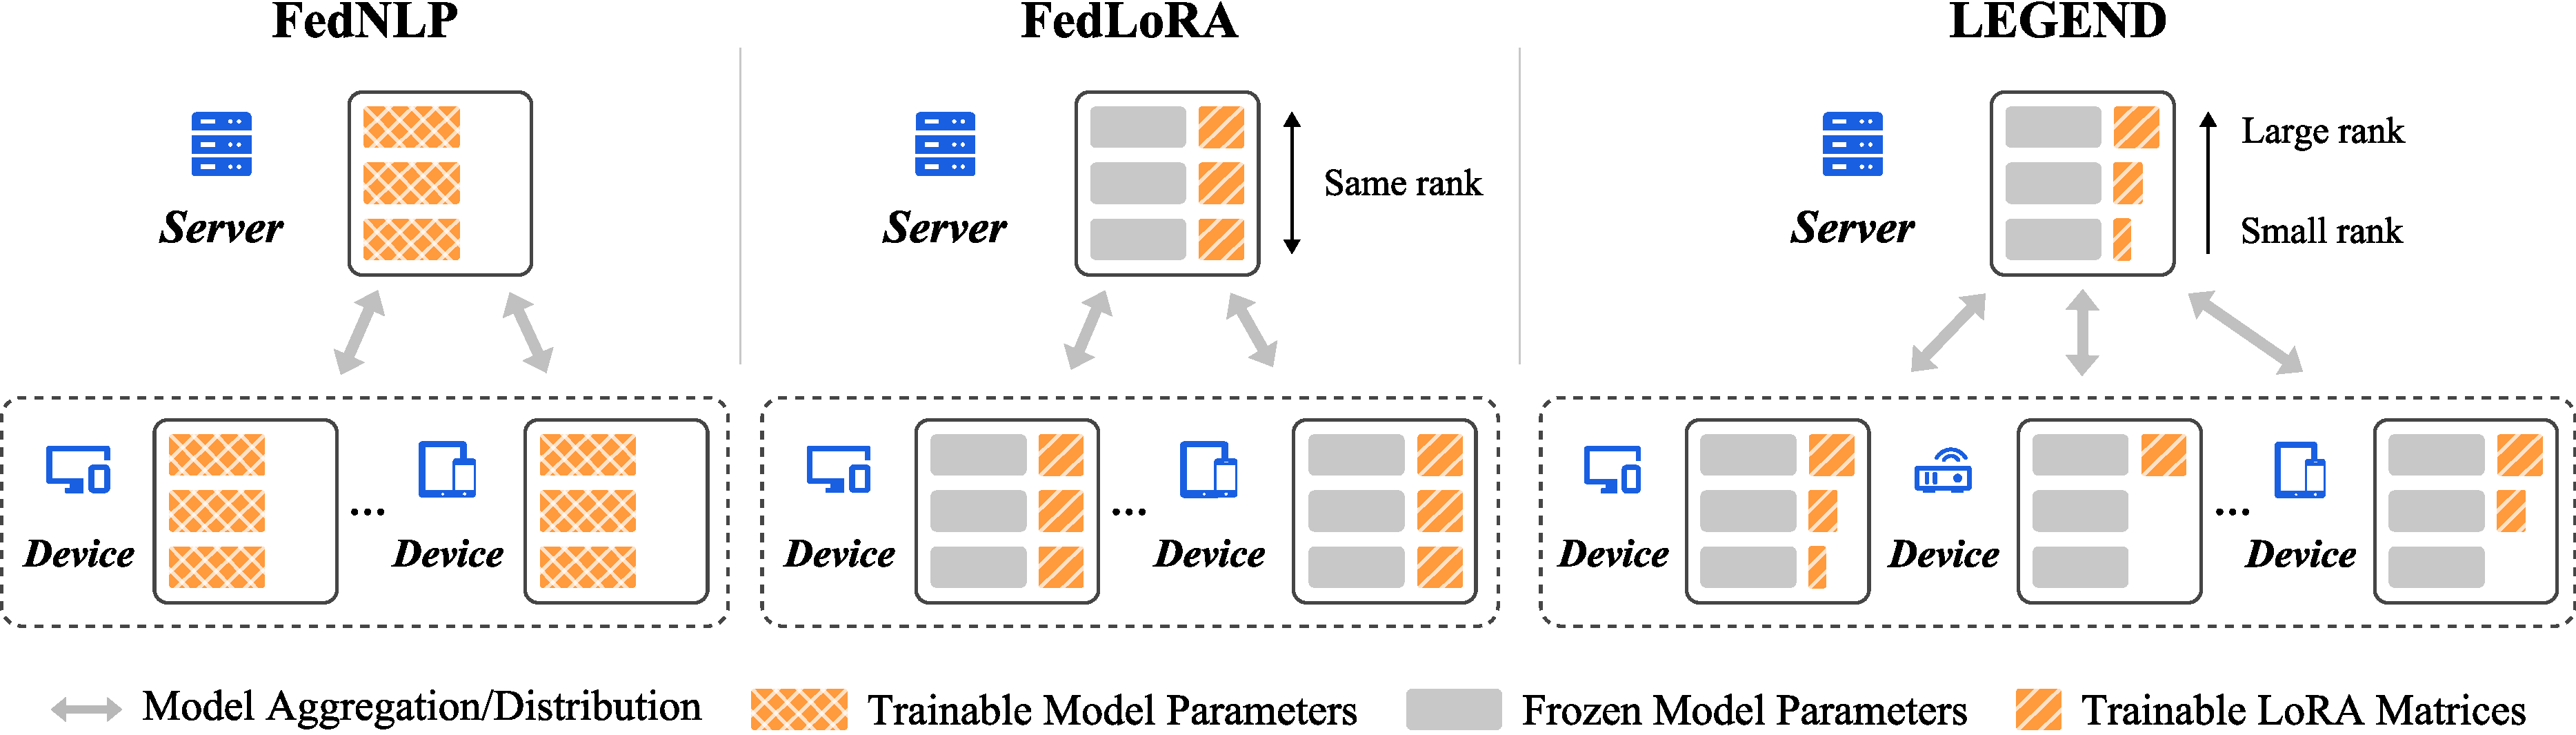
\includegraphics[width=0.99\textwidth]{figs/overview.pdf}
    \vspace{-0.3cm}
    \caption{Illustration of FedNLP, FedLoRA, and LEGEND. 
    FedNLP (left) fine-tunes all parameters of the LM; FedLoRA (mid) applies the same LoRA configuration to all devices; LEGEND (right) applies different LoRA configurations (\eg, LoRA depth) to devices with heterogeneous capabilities.}
    \label{fig:illustration}
    \vspace{-0.4cm}
\end{figure*}

% Motivated by the above insights, LEGEND aims to build up an efficient FedNLP system, which fine-tunes different models with diverse LoRA depths and reasonable rank distribution on heterogeneous devices to deal with resource constraints and system heterogeneity.
% \textbf{The Proposed Framework}

